\documentclass[11pt]{amsart}
\usepackage[margin=1.1in]{geometry}
\usepackage{amsmath,amssymb,amsthm,booktabs,enumitem,graphicx}
\usepackage[colorlinks=true,linkcolor=blue,citecolor=blue,urlcolor=blue]{hyperref}
\graphicspath{{../figures/}}
\allowdisplaybreaks
\setlength{\emergencystretch}{2.5em}
\newtheorem{theorem}{Theorem}[section]
\newtheorem{proposition}[theorem]{Proposition}
\newtheorem{lemma}[theorem]{Lemma}
\newtheorem{corollary}[theorem]{Corollary}
\theoremstyle{remark}
\newtheorem{remark}[theorem]{Remark}
\newcommand{\Z}{\mathbb Z}
\newcommand{\Q}{\mathbb Q}
\newcommand{\e}{\varepsilon}
\newcommand{\cA}{\mathcal A}
\newcommand{\cE}{\mathcal E}
\newcommand{\cP}{\mathcal P}
\newcommand{\fp}{\mathfrak p}
\newcommand{\fa}{\mathfrak a}
\newcommand{\sS}{\mathfrak S}
\DeclareMathOperator{\Cl}{Cl}

\title[Sums of two squares and Heegner norms, XIII]{Sums of two squares and Heegner norms with few prime factors, XIII:\\ half-dimensional vector sieves, class-group covering,\\ and explicit small $r$ for arbitrary class pairs $(C',C)$}
\author{Ruqing Chen}
\address{GUT Geoservice Inc., Montreal, Canada}
\email{ruqing@hotmail.com}
\date{\today\ (draft)}

\begin{document}
\begin{abstract}
Parts~X--XII proved that every large $N$ is $Q_{C'}(u,v)+Q_C(x,y)$ with $Q_{C'}(u,v)$ prime and $\Omega(Q_C(x,y))\le r$. There $r$ is an absolute constant that was never computed: it comes from a sieve of level $N^{\theta_0}$, and $\theta_0$ comes from an unspecified power saving of Assing--Blomer--Li. Moreover the class $C'$ of the prime could be prescribed only for idoneal $D$. Here we replace the weighted count by Iwaniec's half-dimensional sieve. The condition ``$m$ is a norm from $\Q(\sqrt{-D})$'' is detected by sifting out the inert primes. A congruence on $p$ makes $\chi_{-D}(N-p)=1$, and this forces the inert primes to occur in pairs. So only the Bombieri--Vinogradov level $N^{1/2}$ is needed, for the primes $p$, and no weighted sum along $N-p$. We combine two semi-linear sieves (split primes and inert primes) in a vector sieve, remove the pairs of large inert primes by Chen's switching, and add Richert's weights and an iterated Buchstab recursion on the inert primes. The resulting first-order sieve inequality is optimized numerically. For $h(-D)=1$ (nine fields) and every large even admissible $N$ we obtain $N=Q(u,v)_{\rm prime}+Q(x,y)_{P_7}$. The same holds for every idoneal discriminant of Part~XII and every pair $(C',C)$ with $(N-b,D)=1$, with $P_7$ or $P_{7+a}$ where $2^a\parallel N-p$. For $D=23$ ($h=3$) we prescribe both classes: Theorem~\ref{thm:d23} gives $r(C',C)\in\{8,9,11,12,17,18\}$ for all class pairs. An elementary bound for the switched term shows that every switching loss can be absorbed (Proposition~\ref{prop:allL}). So for every prime $D\equiv3\pmod4$ and every pair $(C',C)$ we get an explicit $r(C',C)\le 125\epsilon_{C'}h+h-1$ when $h\le10^7$, and $r(C',C)\ll h\log h$ in general (Corollary~\ref{cor:allD}). The two new inputs are as follows. (i) A Bombieri--Vinogradov theorem, with rational moduli up to $x^{1/2}(\log x)^{-B}$, for the primes represented by a single form $Q_{C'}$. It is proved with Hecke characters $\psi\cdot(\xi\circ{\rm N})$, the classical large sieve, and the convexity bound. (ii) A covering lemma in the class group. If a fixed split prime $q_0$ in a non-principal class divides $m$ exactly to the power $1$ (resp.\ $2$), then $m$ is represented by the non-principal forms (resp.\ by all forms) as soon as all other prime factors of $m$ split. This is a congruence on $p$, so no bad set has to be removed. Obstacle~(1b) of Part~XI is not solved but absorbed: the switched term cannot keep the class of the prime, which costs a factor $L_{C'}\in\{1,\frac32,3\}$; the sieve pays for it with a larger $r$. The numerics check the covering lemma for all $m\le1.1\cdot10^6$ (no failure) and the class-pair counts for $D=23$ near $N=10^6$.
\end{abstract}
\maketitle

\section{Introduction}
This is Part~XIII of the series. For a fundamental discriminant $-D$, a class $C$ of $K=\Q(\sqrt{-D})$ and its reduced form $Q_C$, Parts~X--XII \cite{ChenX,ChenXI,ChenXII} proved statements of the shape
\begin{equation}\label{eq:shape}
N=Q_{C'}(u,v)+Q_C(x,y),\qquad Q_{C'}(u,v)=p\ \text{prime},\qquad \Omega(Q_C(x,y))\le r,
\end{equation}
for every large admissible $N$. In those papers $r=\lceil3/\theta\rceil+O(1)$, where $N^{\theta}$ is the level of distribution of the weighted sequence $r_C(N-p)$. That level rests on the Titchmarsh divisor problem along $N-p$ (Assing--Blomer--Li \cite{ABL}, Part~X) and on its cusp-form analogue (Part~IX \cite{ChenIX}), so $\theta$ is a tiny unspecified constant. The class $C'$ of the prime could be prescribed only when it is a genus condition (Part~XII); for $h>1$ non-idoneal this is obstacle~(1b) of Part~XI.

The point of this paper is that existence in \eqref{eq:shape} does not need the weighted count. Whether $m=N-p$ is a norm depends only on the primes dividing $m$, and that is a sieve condition. This is Iwaniec's approach to $p=a^2+b^2+1$ \cite{Iw72,Iw76}. Recently Nath and Xie \cite{NX} combined it with a linear sieve to make $p+2$ almost prime as well. We run it on $N-p$, where it detects the norm property and the number of prime factors at the same time.

\subsection*{Results}
Throughout, $D$ is $4$, $8$ or a prime $\equiv3\pmod4$; so $h=h(-D)$ is odd when $D>8$. Let $\chi=\chi_{-D}$. For a class $C'$ put $\epsilon_{C'}=2$ if $C'=C'^{-1}$ (for odd $h$ this means $C'$ principal) and $\epsilon_{C'}=1$ otherwise, and
\[
L_{C'}=\tfrac12\epsilon_{C'}h .
\]
So $L_{C'}=1$ if $h=1$, and $L_{C'}\in\{3,\frac32\}$ for the principal and the non-principal classes when $h=3$. A prime $p\nmid D$ is represented by $Q_{C'}$ if and only if $p$ splits and the prime ideals above $p$ lie in $\{C',C'^{-1}\}$. The proportion of such primes among all primes is $1/(\epsilon_{C'}h)$.

\begin{theorem}[Bombieri--Vinogradov for the primes of one form]\label{thm:bv}
Let $C'$ be a class, $b$ a residue modulo $D$ with $\chi(b)=1$, and $\Phi$ a fixed smooth function with compact support in $(0,1)$. Put
\[
\pi_{C'}(x;\Phi;q,a)=\sum_{\substack{p\equiv a\,(q)\\ p=Q_{C'}(u,v)}}\Phi(p/x)\log p .
\]
For every $A>0$ there is $B$ such that
\[
\sum_{\substack{k\le x^{1/2}(\log x)^{-B}\\ (k,D)=1}}\ \max_{\substack{a\bmod kD,\ (a,kD)=1\\ a\equiv b\,(D)}}\Bigl|\pi_{C'}(x;\Phi;kD,a)-\frac1{\phi(k)}\pi_{C'}(x;\Phi;D,b)\Bigr|\ll_{D,\Phi,A}x(\log x)^{-A}.
\]
\end{theorem}
The level is that of the classical theorem. Applied directly, the Bombieri--Vinogradov theorem for ideals of $K$ \cite{Huxley,Wilson} only gives $k\le x^{1/4}$, because ${\rm N}(k\mathcal O_K)=k^2$. Here the rational characters enter through the norm, $\xi\circ{\rm N}$, so the large sieve is the classical one on $\Z$. The cusp-form part uses only the convexity bound for $L(s,\psi\cdot\xi\circ{\rm N})$ (Section~\ref{sec:bv}).

Let $r_0(L)$ be the least $r$ for which we verify the sieve inequality of Proposition~\ref{prop:crit} below, with loss factor $L$ and with the iterated Buchstab bounds of Lemma~\ref{lem:buch}, by a margin that exceeds the discretisation error. Section~\ref{sec:num} gives
\[
r_0(1)=7,\qquad r_0(\tfrac32)=10,\qquad r_0(3)=16 .
\]
The relative margins are $10.1\%$, $12.0\%$ and $7.7\%$; with a one-sided quadrature that errs on the safe side they are $8.9\%$, $9.9\%$ and $2.7\%$. With one Buchstab step the values are $8$, $11$ and $17$, and with the rectangle bounds of the vector sieve alone $8$, $11$ and $18$. For comparison, Nath and Xie \cite{NX} obtain $P_9$ in their (different) problem with the vector sieve and Richert's weights; here the recursion lowers the threshold for $L=1$ from $8$ to $7$.

\begin{theorem}[class number one]\label{thm:h1}
Let $D\in\{3,4,7,8,11,19,43,67,163\}$ and $Q$ the form of discriminant $-D$. Let $N$ be large and \emph{admissible}, i.e.\ there is a residue $b$ modulo $8D$ with $b$ represented by $Q$ $D$-adically and $2$-adically, $\chi(N-b)=1$ and $(b(N-b),D)=1$; the precise local conditions are in Section~\ref{sec:sieve}. If $N$ is even, then $N=Q(u,v)+Q(x,y)$ with $Q(u,v)$ prime and $\Omega(Q(x,y))\le7$. If $N$ is odd, the same holds with $\Omega(Q(x,y))\le8$ for $D\in\{4,7,8\}$ and $\le9$ for $D\in\{3,11,19,43,67,163\}$. The same bounds hold with $Q(u,v)$ replaced by an arbitrary prime $p$, i.e.\ for $N=p+Q(x,y)$; in particular every large even $N$ is $p+x^2+y^2$ with $\Omega(x^2+y^2)\le7$.
\end{theorem}

The idoneal discriminants of Part~XII behave like class number one. There the class of a prime is a congruence, so the switched term keeps it ($L_{C'}=1$). The class of a norm is fixed by its genus characters, so no covering prime $q_0$ is needed.

\begin{theorem}[idoneal discriminants]\label{thm:idoneal}
Let $-D<-4$ be an idoneal fundamental discriminant (one class per genus, Part~XII), $(C',C)$ a pair of classes, and $M_0={\rm lcm}(D,8)$. Let $N$ be large, and suppose there is a residue $b\bmod M_0$ with the following properties:
\begin{itemize}[leftmargin=1.5em]
\item $b$ is a unit in the genus of $C'$, i.e.\ $\chi_{q^*}(b)=e_q(C')$ for all $q\mid D$;
\item $N-b=2^au$ with $u$ a unit modulo $M_0$ and $(N-b,D)=1$;
\item $2^au$ lies in the genus of $C$.
\end{itemize}
Then there are $\gg_DN(\log N)^{-2}$ representations $N=Q_{C'}(u,v)+Q_C(x,y)$ with $Q_{C'}(u,v)$ prime and $\Omega(Q_C(x,y))\le7+a$. In particular $\Omega\le7$ whenever $N-b$ can be taken odd (e.g.\ $N$ even and $D$ odd).
\end{theorem}
The remaining pairs with $A(C',C;N)>0$ in Part~XII are those that force $q\mid N-p$ for some $q\mid D$. They can be treated by also fixing $q^v\parallel N-p$ by a congruence, at the cost of $v$ further prime factors. We do not tabulate them.

\begin{theorem}[$D=23$]\label{thm:d23}
Let $D=23$, $Q_{C_0}=x^2+xy+6y^2$, $Q_{C_1}=Q_{C_2}=2x^2\pm xy+3y^2$. For every large $N$ with $23\nmid N$ and every pair $(C',C)$ there are $\gg N(\log N)^{-2}$ representations $N=Q_{C'}(u,v)+Q_C(x,y)$ with $Q_{C'}(u,v)$ prime and $\Omega(Q_C(x,y))\le r(C',C)$, where
\begin{center}
\begin{tabular}{lcc}
\toprule
 & $C=C_0$ & $C\in\{C_1,C_2\}$\\
\midrule
$p$ arbitrary (no class condition) & $9$ & $8$\\
$C'\in\{C_1,C_2\}$ & $12$ & $11$\\
$C'=C_0$ & $18$ & $17$\\
\bottomrule
\end{tabular}
\end{center}
The third row uses $r_0(3)=16$, whose margin is $7.7\%$ ($2.7\%$ with the one-sided quadrature). With one Buchstab step it is $19$, $18$, and with the rectangle bounds alone $20$, $19$. The first row holds for every large $N$, with $p$ an arbitrary prime. If $23\mid N$ and $C'$ is prescribed, there is no representation with $23\nmid Q_C(x,y)$, since $\chi(N-p)=-\chi(p)=-1$.
\end{theorem}

For general $D$ the same scheme works with the crude bound of Proposition~\ref{prop:allL} in place of the optimisation.

\begin{corollary}[every prime $D\equiv3\pmod4$]\label{cor:allD}
Let $D>3$ be a prime $\equiv3\pmod4$, $h=h(-D)$ and $\Cl(-D)\cong\bigoplus_{i=1}^s\Z/n_i$. For every large even $N$ with $D\nmid N$ and every pair $(C',C)$ there are $\gg_DN(\log N)^{-2}$ representations $N=Q_{C'}(u,v)+Q_C(x,y)$ with $Q_{C'}(u,v)$ prime and
\[
\Omega(Q_C(x,y))\le r_0\bigl(\tfrac12\epsilon_{C'}h\bigr)+\sum_{i=1}^s(n_i-1),
\]
where $r_0(L)\le250L$ for $1\le L\le10^7$ and $r_0(L)\ll L\log 2L$ for all $L\ge1$ (Proposition~\ref{prop:allL}). In particular $r(C',C)\le125\epsilon_{C'}h+h-1\le251h$ for $h\le10^7$. For odd $N$ add $1$ if $2$ splits and $2$ if $2$ is inert.
\end{corollary}

The first row of Theorem~\ref{thm:d23} is Part~X's theorem for $D=23$ with an explicit $r$. Part~X's $r$ is of size $\lceil3/\theta\rceil$ with $\theta\le\delta_{\rm ABL}/50$, i.e.\ of order at least $10^5$ (Section~\ref{sec:remarks}). The second and third rows prescribe the class of the prime when $h=3$, which Part~XII could not do.

\subsection*{Where the class group enters}
Three facts are used.
\begin{enumerate}[leftmargin=2em]
\item \emph{Parity.} For $m$ prime to $D$, $\chi(m)=(-1)^{\#\{\text{inert prime factors, with multiplicity}\}}$. A congruence on $p$ modulo $D$ fixes $\chi(N-p)=1$. Once the inert primes below $N^\theta$, $\theta>\frac14$, are sifted out, $N-p$ has either no inert factor or exactly two (Section~\ref{sec:sieve}).
\item \emph{Covering.} Ideals of norm $m$ have classes $\sum_\ell\{(e_\ell-2j)c_\ell:0\le j\le e_\ell\}$, a signed sumset (Lemma~\ref{lem:cover}). For $h=3$ a prime power $q_0^2$ with $q_0$ in a non-principal class covers the whole group. In general, $\prod_iq_i^{n_i-1}$ with the $q_i$ in generating classes covers the whole group. This is the only place where the class $C$ of the almost-prime side enters, and it costs $a(C)\le h-1$ prime factors ($a(C)\in\{0,1,2\}$ for $h\le3$).
\item \emph{Hecke characters through the norm.} The class of the prime $p$ is detected by the dihedral forms $\vartheta_\psi$ of Part~V \cite{ChenV}. Twisted by $\xi$ modulo $k$, they become the Hecke characters $\psi\cdot(\xi\circ{\rm N})$, whose $L$-functions are entire and have no real zeros near $1$, because $h$ is odd (Theorem~\ref{thm:bv}).
\end{enumerate}
The sieve itself is dimension-free in $D$. With the normalisation of Section~\ref{sec:sieve}, every local factor at $D$, at $2$ and at $q_0$ cancels between the main term and the switched term (Lemma~\ref{lem:norm}). So one optimisation, depending only on $L_{C'}$, serves all $D$.

\section{The class group}\label{sec:class}
Let $\fp\bar\fp=(\ell)$ for a split prime $\ell$, and write $c_\ell=[\fp]$; then $[\bar\fp]=-c_\ell$ (additive notation). Inert primes $\ell$ give the principal ideal $(\ell)$ of norm $\ell^2$. The ramified prime ideal above $D$ is principal when $h$ is odd, being of order dividing $2$.

\begin{lemma}[covering]\label{lem:cover}
Let $m\ge1$ have no inert prime factor to an odd power, and write $m=\prod_\ell\ell^{e_\ell}$. The classes of the ideals of norm $m$ form the set
\[
\Sigma(m)=\sum_{\ell\ \text{split}}\{(e_\ell-2j)c_\ell:\ 0\le j\le e_\ell\}\subseteq\Cl(-D),
\]
and $m$ is represented by $Q_C$ if and only if $\Sigma(m)\cap\{C,C^{-1}\}\ne\emptyset$. Let $h=3$ and let $q_0$ be a split prime in a non-principal class. If every prime factor of $m$ other than $q_0$ is split or ramified, then:
\begin{enumerate}[label=(\alph*)]
\item if $q_0\parallel m$, $m$ is represented by $Q_{C_1}$ $(=Q_{C_2}$ as a set of values$)$;
\item if $q_0^2\parallel m$, $m$ is represented by all three forms.
\end{enumerate}
\end{lemma}
\begin{proof}
An ideal of norm $m$ is $\prod_\ell\fp_\ell^{j}\bar\fp_\ell^{e_\ell-j}$ times the ideals above the inert and ramified primes, which are principal. Its class is $\sum(2j-e_\ell)c_\ell$. The integer $m$ is represented by $Q_C$ iff it is the norm of an ideal in $C$ or $C^{-1}$ \cite[Thm.~7.7]{Cox}. For (a), $\{\pm c\}+x$ meets $\{c,-c\}$ for every $x\in\Z/3$: for $x=0$ it equals $\{\pm c\}$, and for $x=\pm c$ it contains $\mp c$. For (b), $\{2c,0,-2c\}=\Z/3$.
\end{proof}
For $D=23$ the primes $2$ and $3$ split and are not represented by $x^2+xy+6y^2$, so they lie in the non-principal classes. We take $q_0=2$ for odd $N$ and the least non-principal split prime $q_0\nmid N$ (so $q_0\in\{3,13,\dots\}$) for even $N$. The lemma was checked against direct representation counts for all $m\le1.1\cdot10^6$ (Section~\ref{sec:d23}). For a general class group of odd order the same argument gives the following.
\begin{enumerate}[label=(\alph*),start=3]
\item Let $\Cl(-D)\cong\bigoplus_{i=1}^s\Z/n_i$ ($n_i$ odd), and let $q_i$ be split primes whose ideal classes $c_i$ generate the $i$-th summand. If $\prod_iq_i^{n_i-1}\parallel m$ and every other prime factor of $m$ is split or ramified, then $m$ is represented by every form. Indeed $\{(n_i-1-2j)c_i:0\le j\le n_i-1\}$ has $n_i$ elements spaced by $2c_i$. Since $n_i$ is odd, $2$ is invertible modulo $n_i$, so these are all of $\langle c_i\rangle$. The sum over $i$ is the whole group, and adding the class of the remaining ideal changes nothing.
\end{enumerate}
The cost is $\sum_i(n_i-1)\le h-1$ prime factors; it is $h-1$ for a cyclic group.

\section{Proof of Theorem \texorpdfstring{\ref{thm:bv}}{1.1}}\label{sec:bv}
For a split $p=\fp\bar\fp$ and a class character $\psi$ let $c_\psi(p)=\psi(\fp)+\psi(\bar\fp)$, and $c_\psi(p)=0$ for inert $p$. Orthogonality gives, for $p\nmid D$,
\begin{equation}\label{eq:orth}
\mathbf 1[p=Q_{C'}(u,v)]=\frac1{\epsilon_{C'}h}\sum_{\psi}\bar\psi(C')\,c_\psi(p),
\end{equation}
since $\sum_\psi\bar\psi(C')c_\psi(p)=h(\mathbf 1[\fp\in C']+\mathbf 1[\bar\fp\in C'])$. The trivial character gives $c_1(p)=1+\chi(p)$; its contribution is the Bombieri--Vinogradov theorem for the modulus $kD$, with the residue condition $a\equiv b\pmod D$, and it gives the main term. For $\psi\ne1$ the main term is $0$, and we must show
\begin{equation}\label{eq:bvpsi}
\sum_{\substack{k\le Q\\(k,D)=1}}\frac1{\phi(k)}\sum_{\xi\bmod k}\Bigl|\sum_n\Lambda_\psi(n)\,\xi\eta(n)\,\Phi(n/x)\Bigr|\ll x(\log x)^{-A},\qquad Q=x^{1/2}(\log x)^{-B},
\end{equation}
for each character $\eta$ modulo $D$. Here $\Lambda_\psi(n)=\sum_{{\rm N}\fa=n}\Lambda_K(\fa)\psi(\fa)$ are the coefficients of $-L'/L(s,\psi)$, which agree with $c_\psi(p)\log p$ at primes; the prime powers contribute $O(x^{1/2})$ to each inner sum. Now $\sum_n c_\psi(n)\xi\eta(n)n^{-s}=L(s,\psi\cdot(\xi\eta\circ{\rm N}))$ is the $L$-function of a Hecke character of $K$ whose conductor has norm $\le D^2k^2$.

\emph{This Hecke character is not trivial and not real.} If $\psi\cdot(\xi\eta\circ{\rm N})$ were real, then $\psi^2=(\bar\xi\bar\eta\circ{\rm N})^2$ on ideals prime to $kD$. The left side is unramified. A character of the form $\omega\circ{\rm N}$ ($\omega$ Dirichlet) is unramified only if $\omega\in\{1,\chi\}$, and then $\omega\circ{\rm N}=1$. So $\psi^2=1$, impossible for $\psi\ne1$ and $h$ odd. Hence $L(s,\psi\cdot\xi\eta\circ{\rm N})$ is entire, and it has the zero-free region $\sigma>1-c/\log(Dk(|t|+2))$ with no exceptional zero. For $k\le(\log x)^{B}$ this gives the inner sum $\ll x\exp(-c\sqrt{\log x})$, effectively. This replaces the Siegel--Walfisz theorem.

\emph{Large moduli.} Reduce to primitive $\xi$ modulo $k_1\mid k$ in the standard way \cite[Ch.~28]{Davenport}, at a cost of $(\log x)^2$. Apply Vaughan's identity to $-L'/L(s,\psi)$ with parameters $U=V=(\log x)^{C}$. The coefficients $c_\psi$, $\mu_\psi$ (of $1/L(s,\psi)$) and $\Lambda_\psi$ are bounded by $\tau(n)\log n$.

The \emph{bilinear} terms $\sum_{U<m\le x/V}\sum_n\alpha_m\beta_n\xi\eta(mn)\Phi(mn/x)$ are separated with a Mellin transform of $\Phi$ and estimated by the classical large sieve, $\sum_{k_1\le Q_1}\frac{k_1}{\phi(k_1)}\sum^*_\xi|\sum_{n\le X}b_n\xi(n)|^2\ll(Q_1^2+X)\sum|b_n|^2$. As in \cite[Ch.~28]{Davenport} they contribute $\ll(x/Q_1+Q_1x^{1/2}+xU^{-1/2}+xV^{-1/2})(\log x)^{c}$ to the dyadic block $k_1\sim Q_1$ of \eqref{eq:bvpsi}.

The \emph{linear} terms are $\sum_{m\le UV}\alpha_m\sum_nc_\psi(n)(\log n)^j\xi\eta(n)\Phi(mn/x)$, $j\in\{0,1\}$. By Mellin inversion the inner sum is
\[
\frac1{2\pi i}\int_{(2)}(-1)^jL^{(j)}(s,\psi\cdot\xi\eta\circ{\rm N})\,\tilde\Phi(s)\Bigl(\frac xm\Bigr)^sds .
\]
Shift to $\Re s=0$; there are no poles. The functional equation and $|L^{(j)}(1+it)|\ll\log^2(Dk(|t|+2))$ give $|L^{(j)}(it)|\ll Dk(|t|+2)\log^2(Dk(|t|+2))$. Since $\tilde\Phi$ decays rapidly, the inner sum is $\ll Dk_1\log^2x$, uniformly in $m$. The block $k_1\sim Q_1$ then contributes $\ll Q_1UV D(\log x)^3$.

Summing over the blocks, the right side of \eqref{eq:bvpsi} is $\ll x(\log x)^{-A}$ for $B$ large. Note that the smooth weight $\Phi$ is what makes the linear terms harmless. With a sharp cutoff the twisted sums $\sum_{n\le y}c_\psi(n)\xi(n)$ are only $\ll(ky)^{1/2}\log y$ (Wilton's bound and Gauss sums), and the level drops to $x^{1/3}$. All sieve sums below are weighted by $\Phi(p/N)$, with $\Phi\le\mathbf 1_{(0,1)}$ and $\int\Phi$ as close to $1$ as we like, so nothing is lost. \qed

\section{The sieve}\label{sec:sieve}
\subsection{The sequence}
Fix $D$, the classes $C',C$, and $N$ large. Let $a=a(C)$ and $q_0$ be as follows. If $h=1$: for $N$ even, $a=0$; for $N$ odd, $q_0=2$ and $a=1$ when $2$ is not inert ($D\in\{4,7,8\}$), $a=2$ when $2$ is inert. If $D=23$: $a=1$ for $C\ne C_0$, $a=2$ for $C=C_0$, and $q_0$ is as in Section~\ref{sec:class}. Let $M_0$ be $D$ (resp.\ $8$ for $D=4,8$) times $q_0^{a+1}$. When $a=0$ ($h=1$ and $N$ even) there is no $q_0$, and $M_0=D$ (resp.\ $8$). Everything below, including Lemma~\ref{lem:norm}, holds with $q_0^a=1$. For a general prime $D$ (Corollary~\ref{cor:allD}) $q_0^a$ is replaced by $\prod_iq_i^{n_i-1}$. Here $q_i$ is the least split prime $q_i\nmid N$ in a generating class of the $i$-th summand. Then $q_i\ll_D(\log N)^2$, so the moduli $M_0d$ stay below $N^{1/2}(\log N)^{-B}$ when $d\le N^{1/2}(\log N)^{-B-O(h)}$, and the local factors at the $q_i$ cancel as at $q_0$. Let $\mathcal R$ be the set of residues $b$ modulo $M_0$ such that
\begin{itemize}[leftmargin=1.5em]
\item $b$ is a unit and is represented by $Q_{C'}$ locally at $D$ (i.e.\ $\chi(b)=1$; if $p$ is arbitrary, no condition);
\item $(N-b)/q_0^a$ is a unit modulo $M_0/q_0^{a+1}$ and modulo $q_0$, with $\chi((N-b)/q_0^{a})=1$.
\end{itemize}
$N$ is admissible if $\mathcal R\neq\emptyset$; for $D=23$ this means $23\nmid N$ when $C'$ is prescribed, and it is automatic otherwise. Consider
\[
\cA=\bigl\{m=(N-p)/q_0^{a}:\ p\in C',\ p\bmod M_0\in\mathcal R\bigr\},\qquad\text{each $p$ with weight }\Phi(p/N)\log p/\log N,
\]
and write $X$ for its total weight. Every $m\in\cA$ is prime to $M_0$ and has $\chi(m)=1$. Let $\cP_+$ ($\cP_-$) be the split (inert) primes not dividing $M_0N$, and sift
\[
\cP_1=\cP_+\cap[2,z_1),\quad z_1=N^{\eta};\qquad \cP_3=\cP_-\cap[2,z_3),\quad z_3=N^{\theta},\ \tfrac14<\theta<\tfrac12 .
\]
For $\ell\nmid M_0N$ the density of $\ell\mid m$ is $g(\ell)=1/(\ell-1)$. By Theorem~\ref{thm:bv} (or the classical theorem when $p$ is arbitrary), $\cA$ has level of distribution $N^{1/2-\e}$. Both sifting sets have dimension $\kappa=\frac12$.

\subsection{Survivors}
Let $m\in\cA$ have no prime factor in $\cP_1\cup\cP_3$. A prime $\ell\mid N$ can divide $m$ only if $\ell=p$, which we exclude. If $m$ has no inert factor, it is a product of split primes $\ge z_1$, and $q_0^am$ is represented by $Q_C$ by Lemma~\ref{lem:cover} ($h=1$: every such $m$ is a norm). Otherwise $m$ has inert factors $\ge N^\theta$, at most three of them since $4\theta>1$, and an even number since $\chi(m)=1$. So $m=q_1q_2r$ with inert $q_1\le q_2$ and $r$ a product of split primes $\ge z_1$. If $q_1=q_2$, then $m$ is again a norm. Let $\cE$ be the set of $n=q_1q_2r<N/q_0^a$ with $q_1<q_2$; these are the \emph{bad} survivors.

\subsection{The sieve functions}
For $\kappa=\frac12$ (sifting limit $\beta=1$) the functions of the $\beta$-sieve are \cite{Iw76},\cite[Ch.~14]{FI}
\[
F(s)=\frac{2e^{\gamma/2}}{\sqrt{\pi s}}\ (0<s\le2),\qquad f(s)=\frac{e^{\gamma/2}}{\sqrt{\pi s}}\int_1^s\frac{dt}{\sqrt{t(t-1)}}\ (1\le s\le3),
\]
continued by $(\sqrt sF(s))'=\frac1{2\sqrt s}f(s-1)$ $(s>2)$, $(\sqrt sf(s))'=\frac1{2\sqrt s}F(s-1)$ $(s>3)$. Numerically $f,F\to1$ (at $s=39$ both equal $1$ to six decimals), which checks the normalisation.

For two disjoint sifting sets the vector sieve \cite{BF} gives the inequality
\[
\mathbf 1_a\mathbf 1_b\ge\lambda_a^-\lambda_b^++\lambda_a^+\lambda_b^--\lambda_a^+\lambda_b^+ .
\]
It follows from $(\lambda_a^+-\mathbf 1_a)(\lambda_b^+-\mathbf 1_b)\ge0$ and $\lambda^+\ge0$. With levels $z_1^{s_1}z_3^{s_3}=N^{1/2-\e}$ it gives
\begin{gather}
S(\cA,\cP_1\cup\cP_3)\ge XV_1V_3\,\bigl(\Phi(\eta,\theta)+o(1)\bigr),\label{eq:lower}\\
\Phi(\eta,\theta)=\max_{\eta s_1+\theta s_3=1/2}\bigl[f(s_1)F(s_3)+F(s_1)f(s_3)-F(s_1)F(s_3)\bigr],\notag
\end{gather}
where $V_i=\prod_{\ell\in\cP_i}(1-g(\ell))$.

\subsection{Switching}
Every bad survivor $m=n\in\cE$ satisfies $N-q_0^an=p$, prime. It carries the weight $\Phi(p/N)\log p/\log N=\Phi(1-q_0^an/N)(1+o(1))$, and we give $n\in\cE$ the same smooth weight $\Phi(1-q_0^an/N)$. As in Chen's switching \cite{Chen73}, we count them with the linear upper bound sieve on $\{N-q_0^an:n\in\cE\}$, sifting all primes $\ell\nmid 2M_0N$ up to $N^{1/2-\e}$. The level of distribution $N^{1/2-\e}$ of $\cE$ in progressions follows from the Bombieri--Vinogradov theorem for convolutions \cite{Motohashi,BFI1}, since $q_1\in[N^\theta,N^{1/2}]$. With $F_{\rm lin}(1)=2e^\gamma$ we get
\begin{equation}\label{eq:switch}
\#\{\text{bad survivors}\}\le\bigl(2e^{\gamma}+o(1)\bigr)\,|\cE|\,V_{\cE}\bigl(N^{1/2}\bigr) .
\end{equation}
The class condition $p\in C'$ is lost here. It is not a sieve condition on $N-q_0^an$; detecting it would require the weight $r_{C'}(N-q_0^an)$ along the thin set $\cE$, which is obstacle~(1b). Only the congruence $p\bmod M_0\in\mathcal R$ can be kept. Relative to the main term this costs exactly the factor $L_{C'}$ (Lemma~\ref{lem:norm}).

\subsection{Richert's weights}
For $\lambda>0$ and $0<u_0<\frac12$ put
\[
w(m)=1-\lambda\sum_{\substack{\ell\mid m,\ \ell\in\cP_+\\ z_1\le\ell<N^{u_0}}}\Bigl(1-\frac{\log\ell}{u_0\log N}\Bigr).
\]
If $m<N$ is a product of split primes $\ge z_1$ with $w(m)>0$, then $\lambda(\Omega(m)-1/u_0)<1$, so $\Omega(m)<1/\lambda+1/u_0$. Square factors $\ell^2\mid m$ with $\ell\ge z_1$ occur for $O(N^{1-\eta})$ values of $m$ and are negligible. The bad survivors only have to be subtracted with weight $w_+=\max(0,w)\le1$. A bad survivor $m=q_1q_2r$ has inert $q_1,q_2$, so $w(m)=w(r)$. If $1-2\theta\le u_0$, then $r<N^{1-2\theta}\le N^{u_0}$, so every prime factor of $r$ lies in the range $[z_1,N^{u_0})$ of the Richert sum. For squarefree $r$ with $k$ prime factors and $\log r=v\log N$ this gives exactly
\begin{equation}\label{eq:wr}
w(q_1q_2r)=1-\lambda\Bigl(k-\frac v{u_0}\Bigr).
\end{equation}
The weight $w_+$ depends only on $r$. In the bilinear decomposition of $\{N-q_0^a(q_1r)q_2\}$ it is part of the bounded coefficient of $q_1r$, so the Bombieri--Vinogradov theorem for convolutions applies unchanged. The terms $\ell\mid m$ are bounded by the upper vector sieve $\lambda_1^+\lambda_3^+$ on $\cA_\ell$, at level $N^{1/2-\e}/\ell$.

\subsection{Normalisation and the criterion}
\begin{lemma}\label{lem:norm}
Let $\mathcal B=X\sS(N)\kappa_0/\log N$. Here $\kappa_0=\prod_{\ell\mid M_0,\,\ell>2}(1-\frac1\ell)^{-1}$, and $\sS(N)=\prod_{\ell\nmid2M_0N}(1-\frac1{\ell-1})(1-\frac1\ell)^{-1}\prod_{\ell\mid N,\,\ell\nmid 2M_0}(1-\frac1\ell)^{-1}$. Then, as $N\to\infty$,
\begin{align*}
XV_1V_3&=2\mathcal B\cdot\frac{e^{-\gamma}}{\sqrt{\eta\theta}}\,(1+o(1)),\\
(2e^\gamma)\,|\cE|\,V_{\cE}(N^{1/2})&=2\mathcal B\cdot8L_{C'}J(\eta,\theta)\,(1+o(1)),
\end{align*}
where
\[
J(\eta,\theta)=\frac14\Bigl[\int_\theta^{1/2}\frac{da}{a(1-a)}+\sum_{k\ge1}2^{-k}\int P_k(w)\int_{\theta\le a<(1-w)/2}\frac{da}{a(1-a-w)}\,dw\Bigr],
\]
$P_1(w)=w^{-1}\mathbf 1_{w\ge\eta}$, and $P_{k+1}(w)=\frac1{k+1}\int_\eta^{w-k\eta}P_k(w-t)\frac{dt}t$.
\end{lemma}
\begin{proof}
\emph{Sieve factors.} Write $\prod_{\ell<z,\ \ell\in\cP_\pm}(1-\frac1\ell)=a_\pm(\log z)^{-1/2}(1+o(1))$. Since $\prod_{2<\ell<z}(1-\frac1\ell)\sim2e^{-\gamma}/\log z$ and $\cP_+\cup\cP_-$ contains all odd primes not dividing $M_0N$, we get $a_+a_-=2e^{-\gamma}\kappa_0$. Hence $V_1V_3=\sS(N)\,2e^{-\gamma}\kappa_0/(\log N\sqrt{\eta\theta})\,(1+o(1))$; the tails $\ell\ge z_1$ of $\sS$ and the primes $\ell\mid N$, $\ell\ge z_1$, contribute $1+o(1)$. In the switched term $N-q_0^an$ is odd, prime to $q_0$ (as $q_0\nmid N$) and prime to $D$ (as $N-q_0^an\in\mathcal R$). So the upper sieve sifts exactly the odd primes $\ell\nmid M_0N$, and $V_\cE(N^{1/2})=\sS(N)\,2e^{-\gamma}\kappa_0/(\frac12\log N)\,(1+o(1))$.

\emph{Residue classes.} Take $D$ prime (the cases $D=4,8$ are the same with $8$ in place of $D$). Let $\mathcal R'$ be the set of $b\bmod M_0$ such that $N-b\equiv q_0^au$ with $u$ a unit modulo $q_0$ and modulo $D$, and $\chi(u)=1$. There are $(q_0-1)\frac{D-1}2$ such $b$, and $\mathcal R\subseteq\mathcal R'$. By Theorem~\ref{thm:bv}, and because the class of a split $p$ is independent of $p\bmod M_0$ (the Hilbert class field $H$ satisfies $H\cap\Q(\zeta_{M_0})=K$, as $H/K$ is unramified and $\Q(\zeta_{M_0})/K$ is ramified at every prime above $D$ and $q_0$),
\[
X=\frac2{\epsilon_{C'}h}\cdot\frac{\#\mathcal R}{\phi(M_0)}\cdot\frac N{\log N}\,(1+o(1))=\frac1{L_{C'}}\frac{\#\mathcal R}{\phi(M_0)}\frac N{\log N}(1+o(1)).
\]
Here $2/(\epsilon_{C'}h)$ is the density of $C'$ among the split primes, and $\#\mathcal R/\phi(M_0)$ already contains the factor $\frac12$ of $\chi(p)=1$; if $p$ is arbitrary, the factor $1/L_{C'}$ is $1$. By the prime number theorem the number of $n=q_0^aq_1q_2r<N$ is $\frac N{q_0^a\log N}J(1+o(1))$. The factor $\frac14$ is the density of inert primes for $q_1$ and $q_2$, and $2^{-k}$ is that of split primes for the $k$ factors of $r$. The residues $n\bmod M_0$ are equidistributed over the $(q_0-1)\frac{D-1}2$ classes of $N-\mathcal R'$, and the admissible ones are those with $N-n\in\mathcal R$. So
\[
|\cE_{\rm adm}|=\frac N{q_0^a\log N}J\cdot\frac{\#\mathcal R}{(q_0-1)\frac{D-1}2}(1+o(1))=2J\,\frac{\#\mathcal R}{\phi(M_0)}\frac N{\log N}(1+o(1))=2L_{C'}J\,X\,(1+o(1)),
\]
using $\phi(M_0)=(D-1)q_0^a(q_0-1)$. Both $X$ and $|\cE_{\rm adm}|$ carry the weight $\Phi(p/N)$, with $p=N-q_0^an$ in the switched term. By partial summation, each therefore contains the same factor $\int_0^1\Phi(u)\,du$, and this factor cancels; we have suppressed it in the displays. Multiplying by $2e^\gamma V_\cE(N^{1/2})$ gives the second line. The first line is $X\cdot V_1V_3$.
\end{proof}

\begin{proposition}\label{prop:crit}
Let $L\ge1$, $r\ge1$. Suppose that for some $0<\eta<u_0<\frac12$, $\frac14<\theta<\frac12$ and $\lambda>0$ with $\frac1\lambda+\frac1{u_0}\le r+1$,
\[
\mathcal M=\frac{e^{-\gamma}}{\sqrt{\eta\theta}}\Bigl[\Phi(\eta,\theta)-\frac\lambda2\int_\eta^{u_0}\Bigl(1-\frac t{u_0}\Bigr)G(t)\frac{dt}t\Bigr]-8LJ_\lambda(\eta,\theta)>0,
\]
where $G(t)=\min_{\eta s_1+\theta s_3=1/2-t}F(s_1)F(s_3)$. Here $J_\lambda=J$ if $1-2\theta>u_0$, and if $1-2\theta\le u_0$, $J_\lambda$ is $J$ with the $k$-th term weighted by \eqref{eq:wr}:
\begin{multline*}
J_\lambda(\eta,\theta)=\frac14\Bigl[\int_\theta^{1/2}\frac{da}{a(1-a)}\\
+\sum_{k\ge1}2^{-k}\int P_k(v)\max\Bigl(0,1-\lambda\Bigl(k-\frac v{u_0}\Bigr)\Bigr)\int_{\theta\le a<(1-v)/2}\frac{da}{a(1-a-v)}\,dv\Bigr].
\end{multline*}
Then for every large admissible $N$ with $L_{C'}\le L$ there are $\gg N(\log N)^{-2}$ primes $p\in C'$ with $N-p=q_0^am$, where $q_0^am$ is represented by $Q_C$ and $\Omega(m)\le r$.
\end{proposition}
\begin{proof}
By the vector sieve \eqref{eq:lower}, the Richert terms (where the split primes have density $\frac12$, so $\sum_{\ell\in\cP_+}\frac1\ell$ becomes $\frac12\frac{dt}t$), the switching bound \eqref{eq:switch}, applied to the bad survivors with the weight $w_+$ of \eqref{eq:wr}, and Lemma~\ref{lem:norm},
\[
\sum_{\text{good survivors}}w(m)\ \ge\ 2\mathcal B\,(\mathcal M-o(1)) .
\]
A good survivor with $w(m)>0$ has $\Omega(m)<\frac1\lambda+\frac1{u_0}\le r+1$, and $q_0^am$ is represented by $Q_C$ by Lemma~\ref{lem:cover}. Since $\mathcal B\asymp N(\log N)^{-2}$, the claim follows.
\end{proof}

\subsection{Iterated Buchstab steps on the inert primes}
The vector sieve \eqref{eq:lower} spends the level $N^{\eta s_1}$ on the split primes even though $s_3$ is close to $1$, where $f$ is steep. Buchstab's identity on the inert primes moves this hard region into bounds for sub-problems of lower level, and iterating it improves both bounds. For $X>0$, $e>0$ and $0<a<\frac12$ put
\begin{gather*}
\Phi(X;e,a)=\max_{\substack{es_1+as_3=X\\ s_1,s_3\ge1}}\bigl[f(s_1)F(s_3)+F(s_1)f(s_3)-F(s_1)F(s_3)\bigr]^+,\\
G(X;e,a)=\min_{es_1+as_3=X}F(s_1)F(s_3),
\end{gather*}
with $\Phi(X;e,a)=0$ if there are no such $s_1,s_3\ge1$; in particular $\Phi(X;e,a)=0$ for $X\le a$. So $\Phi(\eta,\theta)\le\Phi(\frac12;\eta,\theta)$ and $G(t)=G(\frac12-t;\eta,\theta)$. Put $\Phi_0=\Phi$, $G_0=G$, and for $m\ge1$
\begin{align}
\Phi_m(X;e,a)&=\max_{0<\theta_0\le a}\Bigl[\sqrt{\frac a{\theta_0}}\,\Phi_0(X;e,\theta_0)-\frac12\int_{\theta_0}^{a}\sqrt{\frac ab}\,G_{m-1}(X-b;e,b)\,\frac{db}b\Bigr]\qquad(X>a),\label{eq:recP}\\
G_m(X;e,a)&=\min_{0<\theta_0\le a}\Bigl[\sqrt{\frac a{\theta_0}}\,G_0(X;e,\theta_0)-\frac12\int_{\theta_0}^{a}\sqrt{\frac ab}\,\Phi_{m-1}(X-b;e,b)\,\frac{db}b\Bigr],\label{eq:recG}
\end{align}
with $\Phi_m(X;e,a)=0$ for $X\le a$ and $\Phi_{m-1}(X-b;e,b)=0$ for $X\le b$. The cut $\theta_0=a$ gives the empty integral, so $\Phi_m\ge\Phi_0$ and $G_m\le G_0$.

\begin{lemma}[iterated Buchstab steps]\label{lem:buch}
For every fixed $m\ge0$, Proposition~\ref{prop:crit} remains true with $\Phi(\eta,\theta)$ replaced by $\Phi_m(\frac12;\eta,\theta)$ and $G(t)$ replaced by $G_m(\frac12-t;\eta,\theta)$. Moreover $\Phi_m\ge\Phi_{m-1}$ and $G_m\le G_{m-1}$, so both sequences converge; and as $\eta\to0$, for every $m$, $\Phi_m(X;\eta,a)\to f(X/a)$ and $G_m(X;\eta,a)\to F(X/a)$.
\end{lemma}
\begin{proof}
Let $\cP_3(z)=\cP_-\cap[2,z)$. We prove by induction on $m$ the following statement $(\ast)_m$. Let $d$ be a product of at most $m$ distinct inert primes, $Y=N^{1/2-\e}/d$ the level left for $\cA_d$, and $N^a$ below every prime factor of $d$. Then, with $X=\log Y/\log N$,
\[
\Phi_m(X;\eta,a)-o(1)\ \le\ \frac{S(\cA_d,\cP_1\cup\cP_3(N^a))}{Xg(d)V_1V_3(N^a)}\ \le\ G_m(X;\eta,a)+o(1),
\]
in the sense that each inequality holds up to a remainder which is a sum $\sum_kc_k\,r(k)$ over moduli $k\le N^{1/2-\e}$ with $|c_k|\le\tau(k)^{m+1}$. Here $r(k)$ is the error of $\cA$ in the progression modulo $k$. For $m=0$ this is the vector sieve \eqref{eq:lower} and its upper-bound version $\lambda_1^+\lambda_3^+$, at level $Y$ (so $z_1^{s_1}N^{as_3}=Y$) and with $c_k\in\{0,\pm1\}$; the lower bound is trivial ($S\ge0$) when $X\le a$.

Let $m\ge1$ and $z_0=N^{\theta_0}$ with $0<\theta_0\le a$. Buchstab's identity gives
\[
S(\cA_d,\cP_1\cup\cP_3(N^a))=S(\cA_d,\cP_1\cup\cP_3(z_0))-\sum_{\substack{q\in\cP_-\\ z_0\le q<N^a}}S(\cA_{dq},\cP_1\cup\cP_3(q)).
\]
\emph{The first term.} By $(\ast)_0$ at level $Y$ it is at least $Xg(d)V_1V_3(z_0)(\Phi_0(X;\eta,\theta_0)-o(1))$, and at most the same with $G_0$.

\emph{The terms with $q=N^b$.} The sequence $\cA_{dq}$ has level $Y/q=N^{X-b}$, and $dq$ is a product of at most $m$ inert primes above $q$. By $(\ast)_{m-1}$ the term is at most $Xg(dq)V_1V_3(q)(G_{m-1}(X-b;\eta,b)+o(1))$ and at least $Xg(dq)V_1V_3(q)(\Phi_{m-1}(X-b;\eta,b)-o(1))$, uniformly for $b\in[\theta_0,a]$. For the lower bound of $S(\cA_d,\dots)$ we use the upper bounds of the terms, and conversely. If $X\le a$ there is no upper bound for the terms with $q\ge Y$, and we keep the trivial lower bound $0$.

\emph{Remainders.} The moduli of the terms are $k=qk'$ with $k'\le N^{1/2-\e}/(dq)$ and $|c_{k'}|\le\tau(k')^{m}$. Given $k$, the prime $q$ is one of its prime factors, so the coefficient of $r(k)$ in the sum over $q$ is at most $\omega(k)\tau(k)^m\le\tau(k)^{m+1}$. Theorem~\ref{thm:bv} bounds $\sum_{k\le N^{1/2-\e}}|r(k)|$ by $X(\log N)^{-A}$, and $|r(k)|\ll X\log N/k$ trivially; by Cauchy--Schwarz, $\sum_k\tau(k)^{m+1}|r(k)|\ll X(\log N)^{-A/2+O_m(1)}$, which is $o(X/\log N)$ for $A$ large.

\emph{Normalisation.} By Lemma~\ref{lem:norm}, $V_3(z)=a_-(\log z)^{-1/2}(1+o(1))$, so $V_3(z_0)/V_3(N^a)=\sqrt{a/\theta_0}$ and $V_3(q)/V_3(N^a)=\sqrt{a/b}$. The inert primes have density $\frac12$, so $\sum_{q\in\cP_-}g(q)$ over $N^b\le q<N^{b+db}$ is $\frac12\,db/b$. Dividing by $Xg(d)V_1V_3(N^a)$ and optimising over $\theta_0$ gives \eqref{eq:recP} and \eqref{eq:recG}, i.e.\ $(\ast)_m$.

\emph{The sieve and the Richert terms.} The proposition uses $(\ast)_m$ with $d=1$, $X=\frac12$, $a=\theta$ for the main term, and for the Richert terms the same identity applied to $\cA_\ell$ at level $N^{1/2-\e}/\ell$, with $(\ast)_m$ read with $\cA_\ell$ in place of $\cA$ ($\ell$ is a split prime, so it changes nothing in the induction). The cut $\theta_0$ may depend on $t$ and on the sub-problem. The identity is exact, so the bad survivors and the switched term are unchanged.

\emph{Monotonicity.} $\Phi_1\ge\Phi_0$ and $G_1\le G_0$ by the cut $\theta_0=a$. If $G_{m-1}\le G_{m-2}$, the bracket in \eqref{eq:recP} is at least the bracket of step $m-1$ for every $\theta_0$, so $\Phi_m\ge\Phi_{m-1}$; and likewise $\Phi_{m-1}\ge\Phi_{m-2}$ gives $G_m\le G_{m-1}$. Both sides bound the same counts, so $\Phi_m\le G_0$ and $G_m\ge\Phi_0$, and the monotone sequences converge.

\emph{The limit $\eta\to0$.} Then $f(s_1),F(s_1)\to1$, so $\Phi_0(X;\eta,a)\to f(X/a)$ and $G_0(X;\eta,a)\to F(X/a)$. With $u=X/b$, the substitution $b=X/u$ turns $\frac12\int_{\theta_0}^a\sqrt{a/b}\,F((X-b)/b)\,db/b$ into $\sqrt{a/X}\int_{X/a}^{X/\theta_0}F(u-1)\,du/(2\sqrt u)$, which is $\sqrt{a/\theta_0}f(X/\theta_0)-f(X/a)$ by $(\sqrt sf(s))'=F(s-1)/(2\sqrt s)$. So the bracket in \eqref{eq:recP} with $G_{m-1}=F$ equals $f(X/a)$ for every $\theta_0$, and the bracket in \eqref{eq:recG} with $\Phi_{m-1}=f$ equals $F(X/a)$ by $(\sqrt sF(s))'=f(s-1)/(2\sqrt s)$. Induction on $m$ gives the claim.
\end{proof}
So the recursion gains only through the coupling with the split primes. The same step on the split primes gains nothing at the optima: its terms $G(\frac12-u;u,\theta)$ still sift the inert primes to $N^\theta$ (\texttt{code/nano\_sieve\_probe.py}). If the cuts are restricted to $\theta_0\ge\theta_{\min}$, as on a grid, each step lowers the level of the sub-problems by at least $\theta_{\min}$, so the sequences are constant from $m>1/(2\theta_{\min})+2$ on; numerically they are constant to $10^{-4}$ from $m=10$ on, and we use $m=12$.
The gain comes from the sub-problems. At level $X=\frac12-b$ the ratio $\eta/X$ is three to five times larger than at the top level, so the rectangle bound $G_0(\frac12-b;\eta,b)$ is far from optimal there and a cut improves it: for $\eta=0.008$ and $b=0.35$, $G_0(0.15;\eta,0.35)=2.507$, $G_1=2.484$, $G_2=2.460$, $G_3=2.445$, against $F(0.15/0.35)=2.300$ for $\eta=0$. One step raises $\Phi(\frac12;\eta,\theta)$ by only $0.5$--$0.8\%$ at the optima of the rectangle bounds (cut $\theta_0\approx0.08$), but the recursion compounds, and it moves the optimum to larger $\eta$. At the optima of Table~\ref{tab:r0}, $\Phi_{12}$ exceeds $\Phi_0$ by $8.3\%$, $11.3\%$ and $13.5\%$, and the weighted main term by $20\%$, $25\%$ and $30\%$ ($L=1,\frac32,3$). The thresholds drop from $8,11,18$ (rectangle bounds) to $8,11,17$ ($m=1$) and $7,10,16$ (fixed point).

Theorems~\ref{thm:h1} and~\ref{thm:d23} follow from the proposition and Lemma~\ref{lem:buch} with $r_0(1)=7$, $r_0(\frac32)=10$, $r_0(3)=16$ (Section~\ref{sec:num}) and $\Omega(Q_C(x,y))=a+\Omega(m)$. For $h=1$ and odd $N$ the power of $2$ is fixed by $p\bmod 8$ or $16$: $2\parallel N-p$ if $2$ splits or ramifies, and $4\parallel N-p$ if $2$ is inert.

\emph{Proof of Theorem~\ref{thm:idoneal}.} Take $\mathcal R$ to be the residues $b$ of the theorem, and $q_0^a=2^a$. By Part~XII, $p=Q_{C'}(u,v)$ for a prime $p\nmid D$ iff $p\bmod D$ lies in the genus of $C'$. So $X$ is a sum over primes in residue classes modulo $M_0$, and the classical Bombieri--Vinogradov theorem gives the level $N^{1/2}(\log N)^{-B}$; no cusp form occurs. In the switched term the condition $N-2^an\in\mathcal R$ is again a congruence, and it contains the full condition $p\in C'$. So the computation of Lemma~\ref{lem:norm} gives $|\cE_{\rm adm}|=2JX(1+o(1))$, i.e.\ $L=1$.

In that computation, $n'=q_1q_2r$ is equidistributed modulo $D$ over the units with $\chi(n')=1$, because a product of two primes from the coset $\chi=-1$ is equidistributed over $\ker\chi$. A good survivor $m$ is then a product of split primes, so $2^am$ is the norm of an ideal. Every ideal of norm $2^am$ lies in the genus given by the characters $\chi_{q^*}(2^am)=\chi_{q^*}(N-b)$, which is the genus of $C$, and the genus is the class. So $2^am=Q_C(x,y)$; this is also the pointwise identity $r_C(m)=w\,g(m_{(D)})\mathbf 1[\eta(m)=e(C)]$ of Part~XII \cite[Lemma~2.1]{ChenXII}. Proposition~\ref{prop:crit} with $L=1$ and $r_0(1)=7$ gives the claim. \qed

\subsection{Every loss can be absorbed}
The values in Table~\ref{tab:r0} come from a numerical optimisation. The following crude choice of parameters needs no optimisation and works for every $L$. It uses the unweighted sieve ($\lambda=0$), for which a survivor with no inert factor has $\Omega(m)<1/\eta$.

\begin{proposition}\label{prop:allL}
Let $L\ge1$, $\delta=0.08/L$, $\theta=\frac12(1-\delta)$, $s_3=1+\frac\delta2$. Let $s_1\ge2$ satisfy $F(s_1)-f(s_1)\le0.14\sqrt\delta$, and put $\eta=\delta(1+\delta)/(4s_1)$. Then $\eta s_1+\theta s_3=\frac12$ and
\[
\frac{e^{-\gamma}\Phi(\eta,\theta)}{\sqrt{\eta\theta}}>8LJ(\eta,\theta).
\]
Hence the conclusion of Proposition~\ref{prop:crit} holds with loss $L$ and $\Omega(m)<1/\eta<50Ls_1$. Since $F-f$ is decreasing and $F(5)-f(5)<7.5\cdot10^{-6}$ (Section~\ref{sec:num}), one may take $s_1=5$ for $L\le2.8\cdot10^7$, so $r_0(L)\le250L$ there. Since $F(s)-f(s)\ll e^{-s}$ \cite[Ch.~11]{FI}, one may take $s_1\ll\log2L$ in general, so $r_0(L)\ll L\log 2L$.
\end{proposition}
\begin{proof}
\emph{The level.} $\eta s_1+\theta s_3=\frac{\delta+\delta^2}4+\frac{(1-\delta)(2+\delta)}4=\frac12$. Also $\frac14<\theta<\frac12$ and $\eta<\delta$.

\emph{Upper bound for $J$.} The inner integral $\int_{\theta\le a<(1-w)/2}\frac{da}{a(1-a-w)}$ vanishes unless $w<\delta=1-2\theta$. In that case $a\ge\theta$ and $1-a-w>\frac{1-w}2>\theta$ on the range, which has length $\frac{\delta-w}2$, so the integral is at most $\frac{\delta}{2\theta^2}$. The same bound holds for the term $\int_\theta^{1/2}\frac{da}{a(1-a)}$. Unfolding the recursion,
\[
\int_0^\delta P_k(w)\,dw=\frac1{k!}\int_{\substack{t_1,\dots,t_k\ge\eta\\ t_1+\dots+t_k\le\delta}}\frac{dt_1}{t_1}\cdots\frac{dt_k}{t_k}\le\frac1{k!}\Bigl(\log\frac\delta\eta\Bigr)^k .
\]
Hence
\[
J(\eta,\theta)\le\frac{\delta}{8\theta^2}\sum_{k\ge0}\frac{2^{-k}}{k!}\Bigl(\log\frac\delta\eta\Bigr)^k=\frac{\delta^{3/2}}{8\theta^2\sqrt\eta}.
\]

\emph{Lower bound for $\Phi$.} We have $\Phi\ge f_1F_3+F_1f_3-F_1F_3=F_1f_3-F_3(F_1-f_1)\ge f_1f_3-F_3(F_1-f_1)$, writing $f_i=f(s_i)$, $F_i=F(s_i)$. Here:
\begin{itemize}[leftmargin=1.5em]
\item $f_1\ge f(2)>0.938$;
\item $F_3=2e^{\gamma/2}(\pi s_3)^{-1/2}\le1.506$;
\item by the closed form and ${\rm arsinh}\,y\ge y/\sqrt{1+y^2}$, $f_3\ge2e^{\gamma/2}\pi^{-1/2}\sqrt{s_3-1}/s_3\ge1.02\sqrt\delta$, since $\delta\le0.08$.
\end{itemize}
So $\Phi\ge(0.938\cdot1.02-1.506\cdot0.14)\sqrt\delta>0.745\sqrt\delta$, and the main term is $>0.418\sqrt\delta/\sqrt{\eta\theta}$.

\emph{Comparison.} The inequality follows from $0.418\,\theta^{3/2}>L\delta=0.08$, which holds since $\theta\ge0.46$. Finally $1/\eta<4s_1/\delta=50Ls_1$.
\end{proof}

The two powers $\eta^{-1/2}$ cancel exactly. Both the main term and the switched term are governed by the number of split prime factors $\ge N^\eta$, through $V_1$ and $\sum_k2^{-k}(\log\frac\delta\eta)^k/k!$ respectively. The switched term is small because the two inert primes leave only the room $\delta=1-2\theta$ for the split part. So the loss $L$ is paid for by $\delta\asymp1/L$, i.e.\ by sifting the inert primes almost up to $N^{1/2}$. The optimised parameters show the same law. With the bad survivors at weight $1$, the optima have $L(1-2\theta)=0.210$ for $L=1,\frac32,3$. With the weight \eqref{eq:wr} and the recursion of Lemma~\ref{lem:buch} (Table~\ref{tab:r0}) the values are $0.26$, $0.24$ and $0.24$.

\emph{Proof of Corollary~\ref{cor:allD}.} Since $D$ is prime, $h$ is odd and Theorem~\ref{thm:bv} applies. For $D\ge7$ and $D\nmid N$ there are residues $b$ with $\chi(b)=\chi(N-b)=1$: by a Jacobi sum count their number is exactly $(D-1-2\chi(N))/4\ge(D-3)/4>0$. With $q_0^a$ replaced by $\prod_iq_i^{n_i-1}$, Lemma~\ref{lem:cover}(c) gives the representation by $Q_C$, and Lemma~\ref{lem:norm} holds verbatim. Proposition~\ref{prop:allL} with $L=L_{C'}=\frac12\epsilon_{C'}h\le h$ gives the bound. For odd $N$ the power of $2$ is fixed by a congruence as in Theorem~\ref{thm:h1}. If $2$ splits, its class only shifts the covered set, which is already the whole group. \qed

\section{Numerics: the values of \texorpdfstring{$r_0(L)$}{r0(L)}}\label{sec:num}
The script \texttt{code/semilinear\_sieve.py} computes $f$, $F$, $\Phi$, $G$ and $J$ on grids. The sieve functions use step $10^{-4}$, closed forms on $[1,3]$ and $(0,2]$, and the delay equations beyond. It then maximises $\mathcal M$ over $\eta$, $\theta$ (step $0.005$), $u_0$ (300 values) and $s_1$ (step $0.005$). For one Buchstab step ($m=1$), the cuts $\theta_0$ and the inert primes $q=N^a$ run over a geometric grid of $440$ points in $[0.01,\theta]$ that ends exactly at $\theta$. The integrals are trapezoid sums in $\log a$, and $\Phi(X;e,a)$ and $G(X;e,a)$ are optimised over $500$ and $800$ geometric values of $s_1$.

The recursion \eqref{eq:recP}, \eqref{eq:recG} is computed by \texttt{code/iterated\_buchstab.py} as a two-dimensional dynamic programme on the uniform grid $X=ih$, $a=jh$, $h=1/(2n)$, so that $X-b$ lies on the grid and nothing is interpolated in $X$; the cuts run over the same grid from $\theta_{\min}=h$ on. On each cell $[b_l,b_{l+1}]$ the integrals carry the exact measure $\frac12\int\sqrt{a/b}\,db/b=\sqrt a\,(b_l^{-1/2}-b_{l+1}^{-1/2})$ times the mean of the two endpoint values (trapezoid rule), or times the larger endpoint value in the term subtracted from $\Phi_m$ and the smaller one in the term subtracted from $G_m$ (one-sided rule; it errs on the safe side whenever the integrand is monotone on the cell). $\Phi_0$ and $G_0$ are maxima and minima over $400$ and $600$ geometric values of $s_1$, hence rigorous on every grid, and the Richert integral uses $240$ geometric points with $G_m(\frac12-t;\eta,\theta)$ interpolated linearly in $t$. The production grid is $n=1600$ ($h=1/3200$) with $m=12$ steps.

$J$ changes by at most $0.3\%$ between the grids $2\cdot10^{-3}$, $10^{-3}$ and $5\cdot10^{-4}$:
\begin{itemize}[leftmargin=1.5em]
\item $J(0.008,0.39)=0.3716,\ 0.3711,\ 0.3708$;
\item $J(0.0401,0.3455)=0.3066,\ 0.3058,\ 0.3058$.
\end{itemize}

\begin{table}[htbp]
\centering
\begin{tabular}{cccccccccc}
\toprule
$L$ & $r$ & $\eta$ & $\theta$ & $u_0$ & $1/\lambda$ & main & switched & $\mathcal M$ & $\mathcal M/$main\\
\midrule
$1$ & $7$ & $0.015$ & $0.370$ & $0.329$ & $4.96$ & $2.72$ & $2.44$ & $+0.274\ (+0.238)$ & $10.1\%\ (8.9\%)$\\
$\frac32$ & $10$ & $0.010$ & $0.420$ & $0.268$ & $7.26$ & $2.50$ & $2.20$ & $+0.301\ (+0.242)$ & $12.0\%\ (9.9\%)$\\
$3$ & $16$ & $0.005$ & $0.460$ & $0.199$ & $11.96$ & $2.38$ & $2.19$ & $+0.184\ (+0.062)$ & $7.7\%\ (2.7\%)$\\
\bottomrule
\end{tabular}
\caption{The values $r=r_0(L)$ with the optimal parameters and the fixed point ($m=12$) of Lemma~\ref{lem:buch}, on the grid $n=1600$. ``Main'' is the weighted main term and ``switched'' is $8LJ_\lambda$, both in units of $2\mathcal B$; in parentheses, $\mathcal M$ and $\mathcal M/$main with the one-sided rule. All optima satisfy $1-2\theta\le u_0$. One less fails: $r=6$, $9$, $15$ give $\mathcal M=-0.186$, $+0.018$, $+0.018$ with the trapezoid rule and $-0.223$, $-0.041$, $-0.105$ with the one-sided rule, so $r=9$ and $r=15$ are within the quadrature error and are not claimed. With one Buchstab step ($m=1$) the thresholds are $8$, $11$, $17$, with margins $11.0\%$, $10.1\%$, $2.0\%$; with the rectangle bounds $\Phi$, $G$ they are $8$, $11$, $18$, with margins $9.6\%$, $7.9\%$, $7.7\%$. If moreover the bad survivors carry weight $1$ ($J$ in place of $J_\lambda$), the thresholds are $9$, $12$, $19$.}
\label{tab:r0}
\end{table}
\begin{table}[htbp]
\centering\small\setlength{\tabcolsep}{3.5pt}
\begin{tabular}{cc|cccccc|cc|ccc}
\toprule
& & \multicolumn{6}{c|}{$n=1600$, trapezoid rule} & \multicolumn{2}{c|}{$m=12$} & \multicolumn{3}{c}{$m=12$, one-sided rule}\\
$L$ & $r$ & $m=0$ & $1$ & $2$ & $4$ & $8$ & $12$ & $n=400$ & $800$ & $n=400$ & $800$ & $1600$\\
\midrule
$1$ & $7$ & $-0.179$ & $-0.080$ & $+0.020$ & $+0.187$ & $+0.273$ & $+0.274$ & $+0.268$ & $+0.272$ & $+0.125$ & $+0.201$ & $+0.238$\\
$\frac32$ & $10$ & $-0.203$ & $-0.097$ & $+0.010$ & $+0.193$ & $+0.299$ & $+0.301$ & $+0.287$ & $+0.298$ & $+0.057$ & $+0.181$ & $+0.242$\\
$3$ & $16$ & $-0.359$ & $-0.248$ & $-0.138$ & $+0.052$ & $+0.179$ & $+0.184$ & $+0.137$ & $+0.173$ & $-0.274$ & $-0.066$ & $+0.062$\\
\bottomrule
\end{tabular}
\caption{The margin $\mathcal M$ at the parameters of Table~\ref{tab:r0}: against the number $m$ of Buchstab steps, under refinement of the grid, and with the one-sided cell rule. The column $m=0$ gives the rectangle bounds at these parameters (not at their own optima, which lie at smaller $\eta$). The trapezoid values increase under refinement; the one-sided values converge from below like $h$.}
\label{tab:iter}
\end{table}

Without Richert's weights ($\lambda=0$, $\Omega(m)<1/\eta$) the same computation gives $r=25$ for $L=1$. The weight \eqref{eq:wr} lowers the switched term by $10$--$20\%$; for $L=1$ and $r=8$, it lowers it from $8J=3.89$ to $8J_\lambda=3.21$. This is enough to lower each threshold by one.

The script \texttt{code/prop43.py} checks Proposition~\ref{prop:allL}. On $(0,39]$ the function $F$ never falls below $1$, and $F(s)-f(s)$ is decreasing, with values
\begin{itemize}[leftmargin=1.5em]
\item $0.126$ at $s=2$,
\item $7.1\cdot10^{-3}$ at $s=3$,
\item $2.7\cdot10^{-4}$ at $s=4$,
\item $7.5\cdot10^{-6}$ at $s=5$,
\item $1.3\cdot10^{-7}$ at $s=6$.
\end{itemize}
With the least admissible $s_1$ on a grid of step $0.01$, the proposition gives the bounds
\begin{center}
\begin{tabular}{rrrrrrrrr}
\toprule
$L$ & $1$ & $1.5$ & $3$ & $10$ & $30$ & $100$ & $10^3$ & $10^5$\\
\midrule
$s_1$ & $2.43$ & $2.51$ & $2.63$ & $2.83$ & $3.00$ & $3.20$ & $3.55$ & $4.23$\\
$r_0(L)\le$ & $112$ & $178$ & $384$ & $1403$ & $4488$ & $15987$ & $177485$ & $2.1\cdot10^7$\\
\bottomrule
\end{tabular}
\end{center}
These are far above the optimised values $7,10,16$, but they hold for every $L$. For $L\le100$ the script also evaluates $J$ itself at these parameters. The switched term $8LJ$ is then about $0.6$--$0.7$, against the bound $\approx1.1$ and the main term $\approx2.1$--$2.4$.

The discretisations err on the safe side, and they have converged:
\begin{itemize}[leftmargin=1.5em]
\item $\Phi$ is a maximum over a grid and $G$ a minimum over a grid.
\item The Richert integral, on a geometric grid of $240$ points, increases the margin under refinement. At the three optima the margins for $120,240,480,960$ points agree to $10^{-3}$.
\item $J_\lambda$ changes by at most $0.6\%$ between the grids $10^{-3}$, $5\cdot10^{-4}$ and $2.5\cdot10^{-4}$. For $\eta<0.006$ the grid $10^{-3}$ is too coarse, so the production grid there is $5\cdot10^{-4}$.
\item For one Buchstab step, \texttt{code/check\_richert\_grid.py} refines all grids at once at the optima $r=8,11,17$: the cuts ($440\to880$), the Richert integral ($240\to480$) and $J_\lambda$ ($5\cdot10^{-4}\to2.5\cdot10^{-4}$). The margin increases each time: $+0.397\to+0.399$ ($L=1$), $+0.321\to+0.328$ ($L=\frac32$), $+0.050\to+0.054$ ($L=3$, $r=17$). So that discretisation errs on the safe side by less than $0.01$. The same script checks the one-step identity in the limit $\eta\to0$: for $\theta=0.42$ and $\theta_0=0.1,0.2,0.3$ the bracket in \eqref{eq:recP} equals $0.58471$, $0.58471$, $0.58472$, against $f(1/(2\theta))=0.58474$.
\item \texttt{code/iterated\_buchstab.py} checks the recursion in the limit $\eta\to0$ ($\eta=10^{-7}$): for every $m\le12$ the tables return $f(X/a)$ and $F(X/a)$, and the gain of $m\ge2$ over $m=1$ vanishes. The quadrature error on the unsafe side ($\Phi_m>f$ or $G_m<F$) is at most $3\cdot10^{-4}$ on the grid $n=400$, decreases like $h$, is at most $5\cdot10^{-5}$ at the points used on $n=1600$, and does not grow with $m$; with the one-sided rule it is at most $5\cdot10^{-5}$ already at $n=400$. Multiplied by $e^{-\gamma}/\sqrt{\eta\theta}\le15$ this is below $10^{-3}$ in $\mathcal M$.
\item Under refinement $n=400,800,1600$ the fixed-point margins of Table~\ref{tab:r0} increase, and the one-sided margins increase from below like $h$ and are positive at $n=1600$ for all three rows (Table~\ref{tab:iter}). The unsafe-side error of the trapezoid rule at real $\eta$ is not measured directly; the one-sided values are the certified ones.
\end{itemize}

\begin{remark}\label{rem:18}
At the fixed point the next values fail (one-sided rule, $n=1600$; trapezoid values in parentheses):
\begin{itemize}[leftmargin=1.5em]
\item $r=6$ ($L=1$): $\mathcal M=-0.223$, i.e.\ $-10.4\%$ ($-0.186$);
\item $r=9$ ($L=\frac32$): $\mathcal M=-0.041$, i.e.\ $-1.9\%$ ($+0.018$);
\item $r=15$ ($L=3$): $\mathcal M=-0.105$, i.e.\ $-5.0\%$ ($+0.018$).
\end{itemize}
The trapezoid values of $r=9$ and $r=15$ are positive but within the quadrature error, so they are not claimed. The three cases would pass if the constant $F_{\rm lin}(1)=2e^\gamma$ of the switched term \eqref{eq:switch} were lowered by $9.4\%$, $1.9\%$ and $4.8\%$ respectively. A refined upper bound for $\cE$ might do this, for instance Chen's refinements of the switching constant or a weighted or bilinear upper sieve for $\cE$. A bilinear level $\vartheta>\frac12$ for $\cE$ would lower the constant by the factor $1/(2\vartheta)$. Its prime variable $q_1=N^a$ lies in the balanced range $a\in[\theta,\frac12]\subset[0.37,0.5]$, and we know of no such level for well-factorable weights there. We have not pursued this.
\end{remark}

The margin decreases as $L$ grows, since the switched term grows linearly in $L$. A smaller $\eta$ raises the main term like $\eta^{-1/2}$ but also raises $J$ and the Richert subtraction, and the optimum moves to smaller $\eta$ and larger $\theta$ as $L$ increases. Figure~\ref{fig:margin} shows the margin against $r$.

These are first-order computations. The sieve bounds of Section~\ref{sec:sieve} are asymptotic with $o(1)$ errors, and Siegel's theorem enters through the trivial character of Theorem~\ref{thm:bv}, so ``large $N$'' is ineffective. For comparison, Nath and Xie \cite{NX} obtain $P_9$ in their (different) problem with the same tools.

\section{Numerics for \texorpdfstring{$D=23$}{D=23}}\label{sec:d23}
The script \texttt{code/d23\_classes.py} computes the representation numbers of $x^2+xy+6y^2$ and $2x^2+xy+3y^2$ up to $1.1\cdot10^6$ and checks the following.
\begin{itemize}[leftmargin=1.5em]
\item The classes of the split primes: $2$, $3$ and $13$ are non-principal, and the principal ones make up a proportion $0.3326$ of the split primes in $(10^3,1.1\cdot10^6]$ (expected $\frac13$).
\item Lemma~\ref{lem:cover}: the predicted sets $\Sigma(m)$ agree with the actual representability of $m$ by both forms for all $m\le1.1\cdot10^6$, with no failure.
\item In a sample of $m=N-p$, the $23974$ values with $3\parallel m$ that are norms are all represented by $Q_{C_1}$, and the $8313$ values with $9\parallel m$ are all represented by both forms.
\end{itemize}
Figure~\ref{fig:d23} shows the distribution of $k_{\rm non}(m)$, the number of non-principal prime factors, for the norms $m=N-p$. Without the $q_0$-device the bad sets are large: for $\Omega(m)=1$, a third of the prime values have $k_{\rm non}=0$, and for $\Omega(m)=2$ a third of the values have $k_{\rm non}=1$. Subtracting them by upper bound sieves costs more than the main term. In trial computations (not part of the scripts) the upper bound for the principal-only set was about $7.9$ units of $2\mathcal B$ at $\eta=0.013$, against a weighted main term of about $2.5$; the bound for the set with exactly one non-principal factor was larger still. The congruence $q_0^a\parallel N-p$ avoids this completely.

For every even $N\in[10^6,10^6+400)$ with $23\nmid N$ (192 values), the numbers of $p<N$ with $p\in C'$, $N-p=Q_C(x,y)$ and $\Omega(N-p)\le3$ are at least $1099$ $(C_0,C_0)$, $1898$ $(C_0,C_1)$, $2169$ $(C_1,C_0)$ and $3774$ $(C_1,C_1)$.

\section{Remarks}\label{sec:remarks}
\begin{remark}[Obstacle (1b)]
The class of the prime is detected only in the main term, through Theorem~\ref{thm:bv}. In the switched term it is replaced by the genus condition, with the loss $L_{C'}=\frac12\epsilon_{C'}h$. Proposition~\ref{prop:allL} shows that every finite loss is absorbed: sift the inert primes up to $N^{(1-\delta)/2}$ with $\delta\asymp1/L$. This gives Corollary~\ref{cor:allD} for every prime $D\equiv3\pmod4$ and every pair $(C',C)$, with $r\ll h\log h$. The method never detects prime ideals in a class along a thin set; that problem (obstacle (1b) proper) remains open. What has changed is that, for the existence question, it no longer needs to be solved.
\end{remark}

\begin{remark}[Relation to Parts~X--XII]
The existence statements of Parts~X (for the genus and for $D=23$), XI and XII follow from Theorems~\ref{thm:h1}, \ref{thm:idoneal} and~\ref{thm:d23}, or from the same method, with explicit $r$. For Part~XII this needs the pairs with $(N-b,D)=1$; the others need the extra congruence noted after Theorem~\ref{thm:idoneal}. In Part~X the level was $N^{\theta_0}$ with $\theta_0=\delta/50$, and $\delta$ (from \cite[Prop.~4.1]{ABL}) is not explicit, so $r=\lceil3/\theta\rceil+2E$ was at least of order $10^5$. What the half-dimensional sieve does not give is the asymptotic formula for the weighted counts $\sum_pr_C(N-p)$ along sifted $N-p$, with its local factors. That formula is the content of Parts~VII, IX and~X; for instance, the $199$ exact zeros of Part~XII are statements about it. The two methods answer different questions: the half-dimensional sieve gives existence with small $r$, the spectral method gives the distribution.
\end{remark}

\begin{remark}[What is not covered]
The sieve inequality is optimized numerically at first order, as in Chen-type numerics. A full proof needs, in addition, the level of distribution for the vector sieve with two $\beta$-sieves (as in \cite[Section~3.3]{NX}). It also needs the bilinear Bombieri--Vinogradov theorem for $\cE$, and the trivial treatment of $\ell^2\mid m$, of $\ell\mid N$ and of the small primes. These are standard and do not change the first-order constants. The values of $f$ and $F$ for $\kappa=\frac12$ were taken from \cite{Iw76,FI}, and their normalisation was checked through $f,F\to1$.
\end{remark}

\begin{figure}[htbp]
\centering
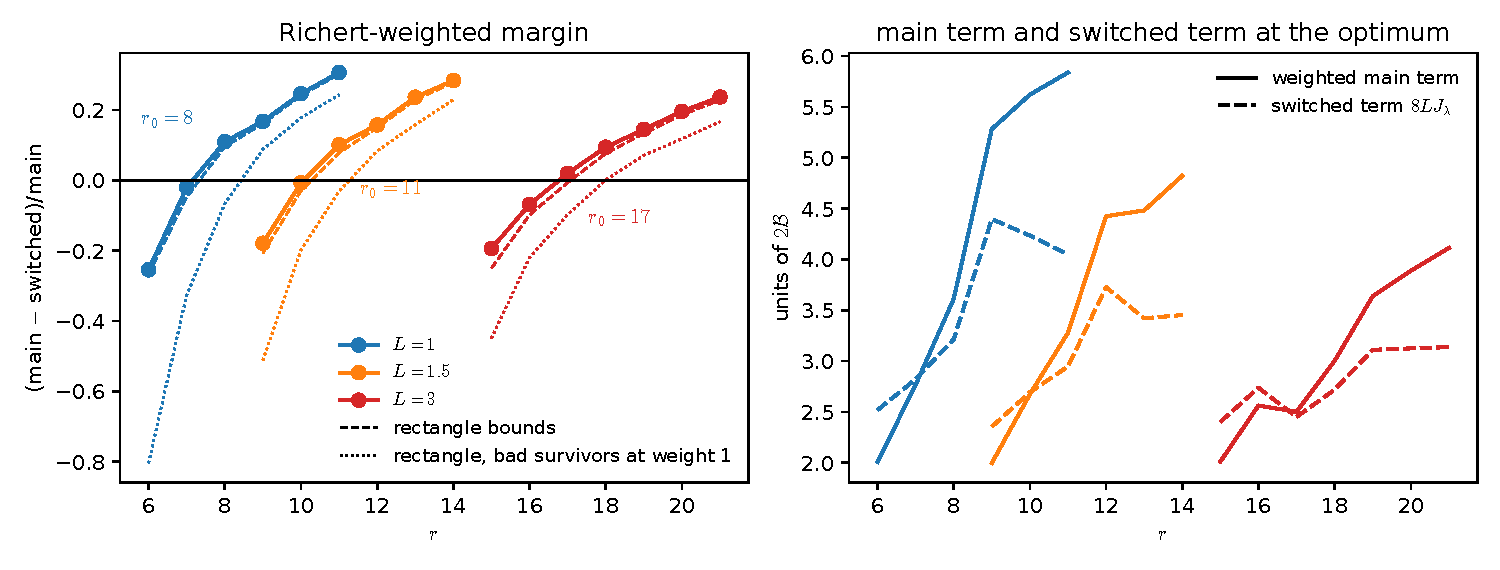
\includegraphics[width=\textwidth]{sieve_margin.pdf}
\caption{Left: the relative margin $\mathcal M/(\text{main})$ of Proposition~\ref{prop:crit} against $r$, for the switching losses $L=1$ ($h=1$, or $p$ without class condition), $L=\frac32$ ($h=3$, $C'$ non-principal) and $L=3$ ($h=3$, $C'$ principal). Solid with markers: the fixed point of Lemma~\ref{lem:buch} ($m=12$, grid $n=400$, trapezoid rule, retuned for each $r$); dash-dotted: one Buchstab step ($m=1$); dashed: rectangle bounds $\Phi$, $G$; dotted: rectangle bounds with the bad survivors at weight $1$. In the first three the bad survivors carry the Richert weight \eqref{eq:wr}. Right: at the fixed-point optimum, the weighted main term (solid) and the switched term $8LJ_\lambda$ (dashed), in units of $2\mathcal B$.}
\label{fig:margin}
\end{figure}

\begin{figure}[htbp]
\centering
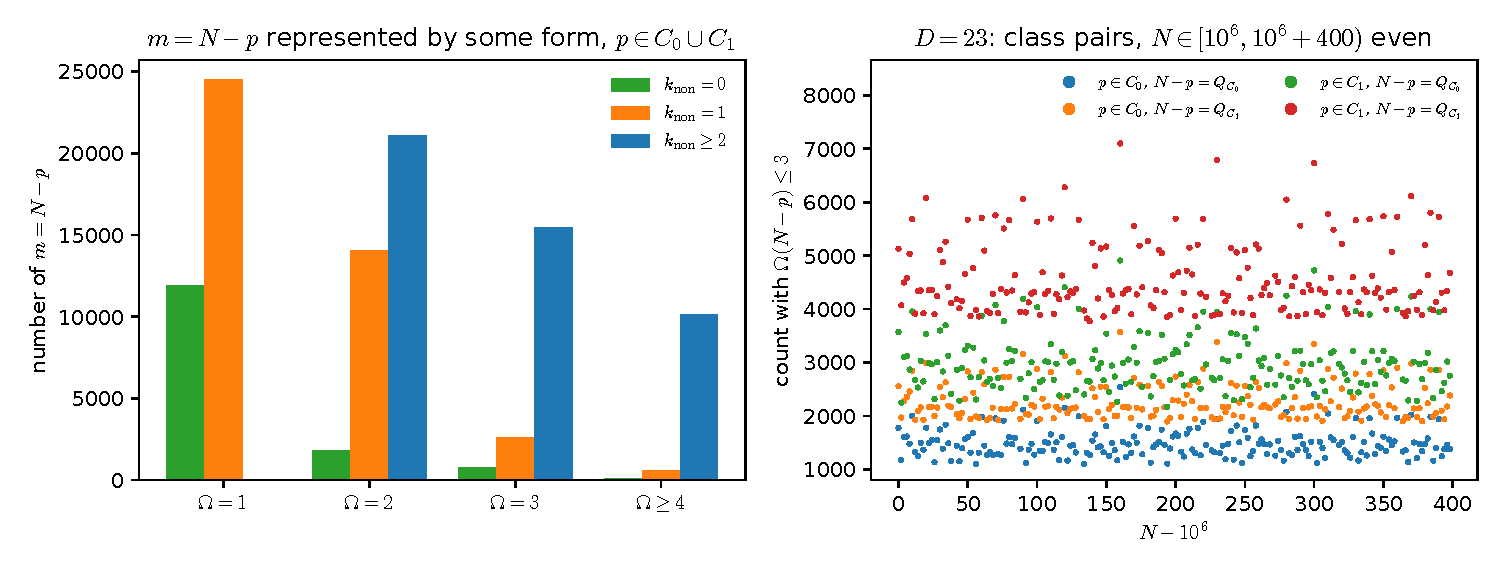
\includegraphics[width=\textwidth]{d23_classes.pdf}
\caption{$D=23$. Left: the norms $m=N-p$ ($p\in C_0\cup C_1$, sampled $N\in[10^6,10^6+400)$) by $\Omega(m)$ and by the number $k_{\rm non}$ of non-principal prime factors; $k_{\rm non}\ge2$ means that $m$ is represented by all three forms. Right: the counts of $p\in C'$ with $N-p=Q_C(x,y)$ and $\Omega(N-p)\le3$, for the four distinct pairs, at every even $N\in[10^6,10^6+400)$ with $23\nmid N$.}
\label{fig:d23}
\end{figure}

\clearpage
\section*{Data and code}
{\raggedright \texttt{code/semilinear\_sieve.py} (Section~\ref{sec:num}; rectangle bounds and one Buchstab step; output \texttt{results/semilinear\_sieve.txt}), \texttt{code/iterated\_buchstab.py} (Section~\ref{sec:num}; the recursion of Lemma~\ref{lem:buch}, with the modes \texttt{fine}, \texttt{safe}, \texttt{safe1600}, \texttt{curve}; outputs \texttt{results/iterated\_buchstab*.txt}), \texttt{code/sieve\_margin\_figure.py} (\texttt{figures/sieve\_margin.pdf}), \texttt{code/check\_richert\_grid.py} (Section~\ref{sec:num}; output \texttt{results/check\_richert\_grid.txt}), \texttt{code/nano\_sieve\_probe.py} (Section~\ref{sec:sieve}; Buchstab steps on the inert and on the split primes; output \texttt{results/nano\_sieve\_probe.txt}), \texttt{code/prop43.py} (Section~\ref{sec:num}; output \texttt{results/prop43.txt}), and \texttt{code/d23\_classes.py} (Section~\ref{sec:d23}; output \texttt{results/d23\_classes.txt}, \texttt{figures/d23\_classes.pdf}). The repository is \url{https://github.com/Ruqing1963/two-squares-vector-sieve}; this paper is archived as doi:10.5281/zenodo.24125302.\par}

\begin{thebibliography}{99}
\bibitem{ABL} E. Assing, V. Blomer, J. Li, Uniform Titchmarsh divisor problems, arXiv:2005.13915 (2020).
\bibitem{BFI1} E. Bombieri, J. B. Friedlander, H. Iwaniec, Primes in arithmetic progressions to large moduli, Acta Math. 156 (1986), 203--251.
\bibitem{BF} J. Br\"udern, \'E. Fouvry, Lagrange's four squares theorem with almost prime variables, J. Reine Angew. Math. 454 (1994), 59--96.
\bibitem{Chen73} J. R. Chen, On the representation of a larger even integer as the sum of a prime and the product of at most two primes, Sci. Sinica 16 (1973), 157--176.
\bibitem{ChenV} R. Chen, Sums of two squares and Heegner norms with few prime factors, V: ideal class groups, weight-one dihedral cusp forms, and the splitting of the scalloped norm, preprint (2026), doi:10.5281/zenodo.23923518.
\bibitem{ChenIX} R. Chen, Sums of two squares and Heegner norms with few prime factors, IX: the dual Titchmarsh divisor problem for weight-one dihedral cusp forms and individual equidistribution of ideal classes, preprint (2026), doi:10.5281/zenodo.24066588.
\bibitem{ChenX} R. Chen, Sums of two squares and Heegner norms with few prime factors, X: the dual Titchmarsh problem in arithmetic progressions and almost prime values of a single ideal class at $N-p$, preprint (2026), doi:10.5281/zenodo.24070749.
\bibitem{ChenXI} R. Chen, Sums of two squares and Heegner norms with few prime factors, XI: split primes, the nine fields of class number one, and $N=Q_{C'}(u,v)_{\rm prime}+Q_C(x,y)_{P_r}$, preprint (2026), doi:10.5281/zenodo.24082184.
\bibitem{ChenXII} R. Chen, Sums of two squares and Heegner norms with few prime factors, XII: idoneal discriminants, genus characters on both sides, and $N=Q_{C'}(u,v)_{\rm prime}+Q_C(x,y)_{P_r}$ for $h>1$, preprint (2026), doi:10.5281/zenodo.24084767.
\bibitem{Cox} D. A. Cox, Primes of the form $x^2+ny^2$, Wiley, New York (1989).
\bibitem{Davenport} H. Davenport, Multiplicative number theory, 3rd ed., Springer GTM 74 (2000).
\bibitem{FI} J. Friedlander, H. Iwaniec, Opera de Cribro, AMS Colloquium Publications 57 (2010).
\bibitem{Huxley} M. N. Huxley, The large sieve inequality for algebraic number fields. III. Zero-density results, J. London Math. Soc. (2) 3 (1971), 233--240.
\bibitem{Iw72} H. Iwaniec, Primes of the type $\phi(x,y)+A$ where $\phi$ is a quadratic form, Acta Arith. 21 (1972), 203--234.
\bibitem{Iw76} H. Iwaniec, The half dimensional sieve, Acta Arith. 29 (1976), 69--95.
\bibitem{Motohashi} Y. Motohashi, An induction principle for the generalization of Bombieri's prime number theorem, Proc. Japan Acad. 52 (1976), 273--275.
\bibitem{NX} R. Nath, Y. Xie, Almost primes and primes that are sums of two squares plus 1, arXiv:2501.16723.
\bibitem{Wilson} R. J. Wilson, The large sieve in algebraic number fields, Mathematika 16 (1969), 189--204.
\end{thebibliography}
\end{document}
